\chapter{Mathematical Documentation}
\label{chapter:mdoc}

The \faust compiler provides a mechanism to produce a self-describing documentation of the mathematical semantic of a \faust program, essentially as a pdf file. The corresponding options are \lstinline!-mdoc! (short) or \lstinline!--mathdoc! (long).

\section{Goals of the mathdoc}
\label{sec:goals-of-mdoc}

There are three main goals, or uses, of this mathematical documentation:
\begin{enumerate}
\item to preserve signal processors, independently from any computer language but only under a mathematical form;
\item to bring some help for debugging tasks, by showing the formulas as they are really computed after the compilation stage;
\item to give a new teaching support, as a bridge between code and formulas for signal processing.
\end{enumerate}

\section{Installation requirements}
\label{sec:inst-requ}

\begin{itemize}
\item \lstinline!faust!, of course!
\item \lstinline!svg2pdf! (from the Cairo 2D graphics library), to convert block-diagrams, as \latex doesn't eat \svg directly yet...
\item \lstinline!breqn!, a \latex package to handle automatic breaking of long equations,
\item \lstinline!pdflatex!, to compile the \latex output file.
\end{itemize}


\section{Generating the mathdoc}
\label{sec:generating-mdoc}

The easiest way to generate the complete mathematical documentation is to call the \lstinline!faust2mathdoc! script on a \faust file, as the \lstinline!-mdoc! option leave the documentation production unfinished. For example: 
\begin{lstlisting}
faust2mathdoc noise.dsp
\end{lstlisting}

\subsection{Invoking the -mdoc option}
\label{sec:invoking-mdoc}

Calling directly \lstinline!faust -mdoc! does only the first part of the work, generating:
\begin{itemize}
\item a top-level directory, suffixed with "\texttt{-mdoc}",
\item 5 subdirectories (\lstinline!cpp/!, \lstinline!pdf/!, \lstinline!src/!, \lstinline!svg/!, \lstinline!tex/!),
\item a \latex file containing the formulas,
\item \svg files for block-diagrams.
\end{itemize}

At this stage:
\begin{itemize}
\item \lstinline!cpp/! remains empty,
\item \lstinline!pdf/! remains empty,
\item \lstinline!src/! contains all \faust sources used (even libraries),
\item \lstinline!svg/! contains \svg block-diagram files,
\item \lstinline!tex/! contains the generated \latex file.
\end{itemize}

\subsection{Invoking faust2mathdoc}
\label{sec:invok-faust2m}

The \lstinline!faust2mathdoc! script calls \lstinline!faust --mathdoc! first, then it finishes the work:
\begin{itemize}
\item moving the output C++ file into \lstinline!cpp/!,
\item converting all \svg files into pdf files (you must have \lstinline!svg2pdf! installed, from the Cairo 2D graphics library),
\item launching \lstinline!pdflatex! on the \latex file (you must have both \lstinline!pdflatex! and the \lstinline!breqn! package installed),
\item moving the resulting pdf file into \lstinline!pdf/!.
\end{itemize}

\subsection{Online examples}
\label{sec:mdoc-examples}

To get an idea of the results of this mathematical documentation, which captures the mathematical semantic of \faust programs, you can look at two pdf files online:
\begin{itemize}
\item \myurl{http://faust.grame.fr/pdf/karplus.pdf} (automatic documentation),
\item \myurl{http://faust.grame.fr/pdf/noise.pdf} (manual documentation).
\end{itemize}

You can also generate all \emph{mdoc} pdfs at once, simply invoking the \lstinline!make mathdoc! command inside the \lstinline!examples/! directory: 
\begin{itemize}
\item for each \lstinline!%.dsp! file, a complete \lstinline!%-mdoc! directory will be generated,
\item a single \lstinline!allmathpdfs/! directory will gather all the generated pdf files.
\end{itemize}


\section{Automatic documentation}
\label{sec:auto-docum}

By default, when no \lstinline!<mdoc>! tag can be found in the input \faust file, the \lstinline!-mdoc! option automatically generates a \latex file with four sections:
\begin{enumerate}
\item ''\textbf{Equations of process}'', gathering all formulas needed for \lstinline!process!,
\item ''\textbf{Block-diagram schema of process}'', showing the top-level block-diagram of \lstinline!process!,
\item ''\textbf{Notice of this documentation}'', summing up generation and conventions information,
\item ''\textbf{Complete listing of the input code}'', listing all needed input files (including libraries).
\end{enumerate}


\section{Manual documentation}
\label{sec:manual-mdoc}

You can specify yourself the documentation instead of using the automatic mode, with five xml-like tags. That permits you to modify the presentation and to add your own comments, not only on \lstinline!process!, but also about any expression you'd like to. Note that as soon as you declare an \lstinline!<mdoc>! tag inside your \faust file, the default structure of the automatic mode is ignored, and all the \latex stuff becomes up to you!

\subsection{Six tags}
\label{sec:doc-tags}

Here are the six specific tags:
\begin{itemize}
\item \lstinline!<mdoc></mdoc>!, to open a documentation field in the \faust code,
  \begin{itemize}
  \item \lstinline!<equation></equation>!, to get equations of a \faust expression,
  \item \lstinline!<diagram></diagram>!, to get the top-level block-diagram of a \faust expression,
  \item \lstinline!<metadata></metadata>!, to reference \faust metadatas (cf. declarations), calling the corresponding keyword,
  \item \lstinline!<notice />!, to insert the "adaptive'' notice all formulas actually printed,
  \item \lstinline!<listing [attributes] />!, to insert the listing of \faust files called.
  \end{itemize}
\end{itemize}

The \lstinline!<listing />! tag can have up to three boolean attributes (set to \lstinline!"true"! by default):
\begin{itemize}
\item \lstinline'mdoctags' for \lstinline'<mdoc>' tags;
\item \lstinline'dependencies' for other files dependencies;
\item \lstinline'distributed' for the distribution of interleaved \faust code between \lstinline'<mdoc>' sections.
\end{itemize}


\subsection{The mdoc top-level tags}
\label{sec:mdoc-tag}

The \lstinline!<mdoc></mdoc>! tags are the top-level delimiters for \faust mathematical documentation sections. This means that the four other documentation tags can't be used outside these pairs (see section \ref{sec:documentation}).

In addition of the four inner tags, \lstinline!<mdoc></mdoc>! tags accept free \latex text, including its standard macros (like \lstinline!\section!, \lstinline!\emph!, etc.). This allows to manage the presentation of resulting tex file directly from within the input \faust file. 

The complete list of the \latex packages included by \faust can be found in the file \lstinline!architecture/latexheader.tex!.

\subsection{An example of manual mathdoc}
\label{sec:ex-mathdoc}

\footnotesize
\begin{lstlisting}
<mdoc>
\title{<metadata>name</metadata>}
\author{<metadata>author</metadata>}
\date{\today}
\maketitle

\begin{tabular}{ll}
	\hline
	\textbf{name}		& <metadata>name</metadata> \\
	\textbf{version} 	& <metadata>version</metadata> \\
	\textbf{author} 	& <metadata>author</metadata> \\
	\textbf{license} 	& <metadata>license</metadata> \\
	\textbf{copyright} 	& <metadata>copyright</metadata> \\
	\hline
\end{tabular}
\bigskip
</mdoc>
//-----------------------------------------------------------------
// Noise generator and demo file for the Faust math documentation
//-----------------------------------------------------------------

declare name 		"Noise";
declare version 	"1.1";
declare author 		"Grame";
declare author 		"Yghe";
declare license 	"BSD";
declare copyright 	"(c)GRAME 2009";

<mdoc>
\section{Presentation of the "noise.dsp" Faust program}
This program describes a white noise generator with an interactive volume, using a random function.

\subsection{The random function}
</mdoc>

random  = +(12345)~*(1103515245);

<mdoc>
The \texttt{random} function describes a generator of random numbers, which equation follows. You should notice hereby the use of an integer arithmetic on 32 bits, relying on integer wrapping for big numbers.
<equation>random</equation>

\subsection{The noise function}
</mdoc>

noise   = random/2147483647.0;

<mdoc>
The white noise then corresponds to:
<equation>noise</equation>

\subsection{Just add a user interface element to play volume!}
</mdoc>

process = noise * vslider("Volume[style:knob]", 0, 0, 1, 0.1);

<mdoc>
Endly, the sound level of this program is controlled by a user slider, which gives the following equation: 
<equation>process</equation>

\section{Block-diagram schema of process}
This process is illustrated on figure 1.
<diagram>process</diagram>

\section{Notice of this documentation}
You might be careful of certain information and naming conventions used in this documentation:
<notice />

\section{Listing of the input code}
The following listing shows the input Faust code, parsed to compile this mathematical documentation.
<listing mdoctags="false" dependencies="false" distributed="true" />
</mdoc>
\end{lstlisting}
\normalsize

The following page which gathers the four resulting pages of \lstinline!noise.pdf! in small size. might give you an idea of the produced documentation.


\subsection{The -stripmdoc option}
\label{sec:striping-option}

As you can see on the resulting file \lstinline!noisemetadata.pdf! on its pages 3 and 4, the listing of the input code (section\,4) contains all the mathdoc text (here colored in grey). As it may be useless in certain cases (see Goals, section \ref{sec:goals-of-mdoc}), we provide an option to strip mathdoc contents directly at compilation stage: \lstinline!-stripmdoc! (short) or \lstinline!--strip-mdoc-tags! (long).


\section{Localization of mathdoc files}
\label{sec:localization-mdoc}

By default, texts used by the documentator are in English, but you can specify another language (French, German and Italian for the moment), using the \lstinline!-mdlang! (or \lstinline!--mathdoc-lang!) option with a two-letters argument (\lstinline!en!, \lstinline!fr!, \lstinline!it!, etc.).

The \lstinline!faust2mathdoc! script also supports this option, plus a third short form with \lstinline!-l!:
\begin{lstlisting}
faust2mathdoc -l fr myfaustfile.dsp
\end{lstlisting}

If you would like to contribute to the localization effort, feel free to translate the mathdoc texts from any of the \lstinline!mathdoctexts-*.txt! files, that are in the \lstinline!architecture! directory (\lstinline!mathdoctexts-fr.txt!, \lstinline!mathdoctexts-it.txt!, etc.). As these files are dynamically loaded, just adding a new file with an appropriate name should work.

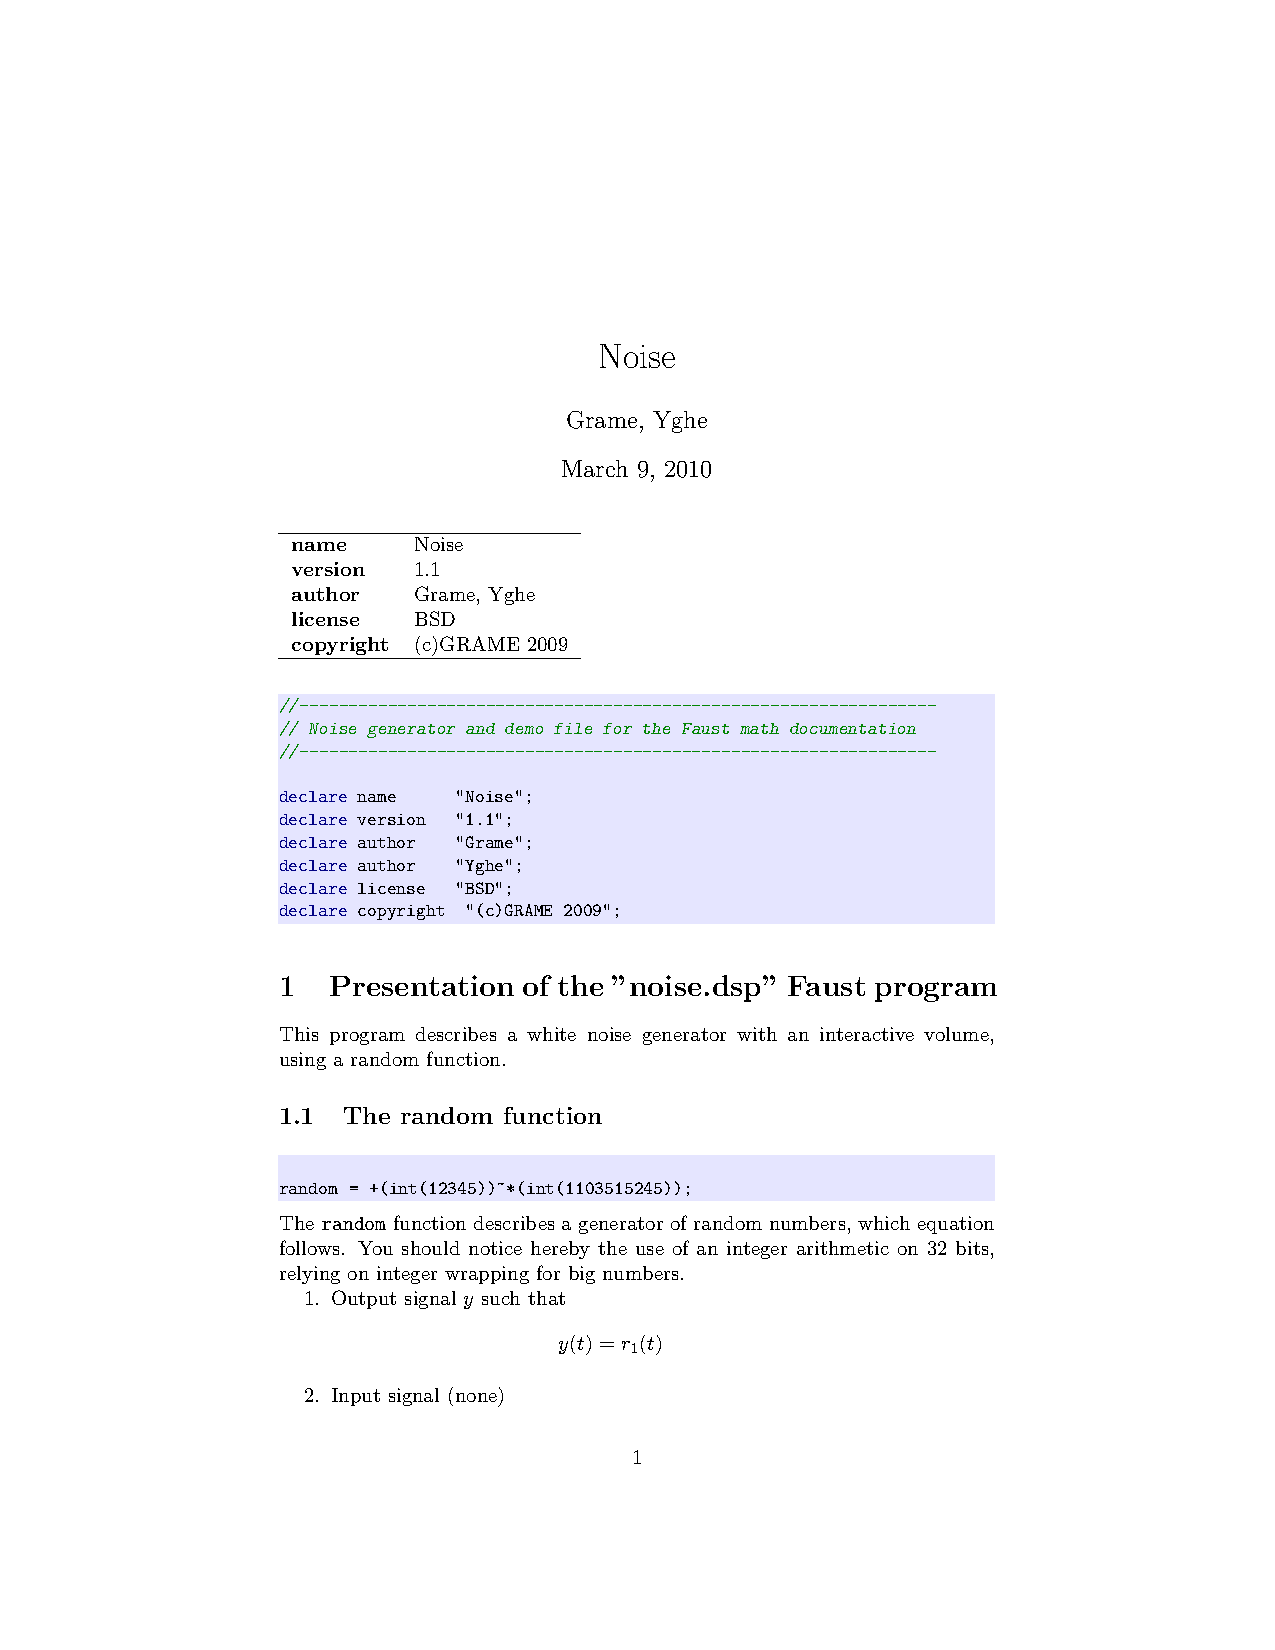
\includepdf[pages=-, frame=true, angle=-90, scale=0.75, nup=1x2]{images/noisemetadata}


\section{Summary of the mathdoc generation steps}
\label{sec:mdoc-summary}

\begin{enumerate}
\item First, to get the full mathematical documentation done on your faust file, call \lstinline!faust2mathdoc myfaustfile.dsp!.
\item Then, open the pdf file \lstinline!myfaustfile-mdoc/pdf/myfaustfile.pdf!.
\item That's all !
\end{enumerate}



